\documentclass[a4paper,10pt,oneside,fleqn]{jsbook}
%
\usepackage{amsmath,amssymb,bm}
\usepackage{bm}
\usepackage{graphicx}
\usepackage{ascmac}
\usepackage{makeidx}
\usepackage{txfonts}
\usepackage{indentfirst}
\usepackage{indent}
\usepackage{booktabs}
\usepackage{comment}
\usepackage{cite}
\usepackage{ulem}
\usepackage{alltt}
\usepackage{eclbkbox,fancybox}

% プログラム環境
\newcounter{program}
%\bkcounttrue
\newenvironment{program}%
{\vspace{0.5\baselineskip}\VerbatimEnvironment%
%\begin{breakbox}\setlength{\baselineskip}{0pt}\begin{Verbatim}}%
\begin{breakbox}\setlength{\baselineskip}{.25\normalbaselineskip}\begin{Verbatim}}%
{\end{Verbatim}\end{breakbox}\vspace{0.8\baselineskip}}

%
\makeindex
%
\newcommand{\diff}{\mathrm{d}}  %微分記号
\newcommand{\divergence}{\mathrm{div}\,}  %ダイバージェンス
\newcommand{\grad}{\mathrm{grad}\,}  %グラディエント
\newcommand{\rot}{\mathrm{rot}\,}  %ローテーション
%
\setlength{\textwidth}{\fullwidth}
\setlength{\textheight}{44\baselineskip}
\addtolength{\textheight}{\topskip}
\setlength{\voffset}{-0.6in}
\setlength{\mathindent}{1.5cm} %数式のインデント設定
\setcounter{secnumdepth}{2} %subsectionまで番号付け
\setcounter{tocdepth}{2} %目次の深さ設定
\renewcommand\citemid{; } %citeのオプション

%
\usepackage{atbegshi}
\AtBeginShipoutFirst{\special{pdf:tounicode EUC-UCS2}}
\usepackage[dvipdfm,bookmarks=true,bookmarksnumbered=true]{hyperref}
%
\begin{document}

\begin{titlepage}
\begin{center}
\vspace*{3cm}
{\huge \textbf{User Guide of V-Sphere}}\\
\vspace{1cm}

{\large \textbf{Ver. 1.2.2}}\\
\vspace{1.5cm}

{\large \textbf{Functionality Simulation and Information Team}\\
\large \textbf{VCAD System Research Program}\\
\large \textbf{RIKEN}\\
\vspace{1cm}
}

{\large 2-1, Hirosawa, Wako, 351-0198, Japan}\\
\vspace{0.5cm}

{http://vcad-hpsv.riken.jp/}\\
\vspace{1cm}

June 2011\\
\vspace{4cm}


\includegraphics[width=4cm,bb=-80 0 220 500]{RIKEN_logo_300x500.png}

\end{center}
\end{titlepage}
\newpage


%
\frontmatter

\begin{tabular}{lllr}
First Edition  &  version 1.0.0  &  5 Mar.  &  2009\\
               &  version 1.1.0  &  5 Jan.  &  2010\\
               &  version 1.2.0  & 10 May   &  2011\\
               &  version 1.2.1  &  6 June  &  2011\\
               &  version 1.2.2  & 20 June  &  2011
\end{tabular}

\vspace{14cm}

\begin{description}
\item[ ] \textbf{COPYRIGHT}\\
(c) Copyright RIKEN 2007-2011. All rights reserved.\\

\item[ ] \textbf{DISCLAIMER}\\
You shall comply with the conditions of the license when you use this program.\\
The license is available at http://vcad-hpsv.riken.jp/permission.html
\end{description}
%

\tableofcontents
%
%
\mainmatter

%%%
\chapter{イントロダクション}
{\begin{abstract}
物理現象の解析や工業製品の設計のため,シミュレーションは不可欠な技術となっている.特に,製品開発ではコストや性能の検討のため,高精度な計算結果を迅速に得たいというエンジニアの要求が高くなっている.また,複雑な物理現象の解明のため,異なる物理現象の連成解析や非線形マルチスケール現象を扱うシミュレーション研究が進んでいる.これらの先端的な研究は,必然的に分散並列の大規模解析となる傾向にある.
従来から,流体解析や構造解析では領域分割型の並列計算法が研究され,並列化粒度の大きな効率のよい計算手法が提案されてきた.これらはMPIを用いた並列プログラムであるが,デバッグを含めたコード開発とメンテナンスが難しい点が問題であり,開発支援の仕組みが必要となっている.
この問題点を緩和する目的のために,オブジェクト指向プログラミング\index{おぶじぇくとしこうぷろぐらみんぐ@オブジェクト指向プログラミング}(Object-Oriented Programming\index{Object-Oriented Programming}, OOP)によるクラスライブラリ,フレームワークなどの並列プログラミング支援環境が研究されてきた.

この章では,OOPを用いて構築された様々な物理現象シミュレータ開発のためのフレームワークV-Sphereの概要について述べる.
\end{abstract}
%

\graphicspath{{./fig1/}}

\section{V-Sphereとソルバークラス}
\label{sec:1.1}
複数の物理ソルバを連成したマルチフィジックス解析では,複数ソルバの実行制御・管理の問題が顕在化している.物理シュミレーションの数値解法は,各々の現象に対して効率のよい固有の解法として発展し,専門性の強い研究領域を形成している.一人の研究者で全ての現象解析をカバーすることは難しいため,連成解析のシステム開発にあたり,研究者間のコラボレーションを促進する仕組みには大きな期待が寄せられている.具体的には,プログラム開発のガイドライン,あるいは共通機能を持つフレームワークを利用することにより,開発効率やプログラムの品質の向上を図ることができる.特に,大規模なソフトウェア,複数のプログラマによる協同作業の場合には,作業効率やメンテナンス性の点からはこれらの仕組みが必須である.

プログラムの開発支援と実行管理の問題点に対して,著者らは物理シミュレーションのひな型の提供と複数のソルバーコードを管理し,選択・連成実行可能なアプリケーションの機能を持つオブジェクト指向フレームワークV-Sphereを提案している~\cite{ono:V-SphereJSCES, ono:V-SphereACS18, ono:SphereParCFD08}.
このフレームワークは,オブジェクト指向技術の積極的な利用により,非定常/定常物理シミュレーションのソフトウェア構造の標準化・統一化を推進している.また,アプリケーションの開発効率化・高品質化・メンテナンス性の向上に貢献し,先端シミュレーション技術の迅速なパッケージングが期待できる.

V-Sphere\index{V-Sphere}は,非定常物理シミュレーションのフレームワークとして設計されている.
V-Sphereフレームワークは,\textbf{図\ref{fig:V-Sphere_framework}}に示す様々なライブラリ機能と\textbf{図\ref{fig:Control_structure}}に示す非定常物理現象のシミュレータに共通する制御構造をソルバー開発者に提供する.
つまり,時間的に変化する物理現象の解析プログラムはどれも同様に記述できる点に着目し,処理の大まかな流れ(前処理,本計算,後処理の3つのステージ)を規定し,共通機能を抽出し,APIとしてまとめている.
制御構造はSklSolverBase\index{SklSolverBase}クラスに内包されており,開発者はこのソルバー基底クラスを継承したクラスを作成し,この派生クラスにユーザ関数・サブルーチンをクラスメソッドとして実装することによりプログラムを作成する.
また,通常の意味でのサブルーチンも多く用意し,計算パラメータなどの入力データ,計算結果の入出力などの機能を提供している.
これらの利用により,ソルバ開発者にとって本質的でないプログラミングを減らし,開発の効率化が期待できる.
システムの実装はオブジェクト指向に基づきC++で記述されているが,従来資産の移行,物理コードの開発者がCやFortran言語を使い慣れていることを考慮し,プログラミングモデルとしては手続き型言語の記述を基本としている.具体的には,Fortran/C言語へのインタフェースを備えている.

\begin{figure}[htbp]
\begin{center}
\includegraphics[width=12cm,clip]{V-Sphere_framework.eps}
\end{center}
\caption{V-Sphere frameworkのブロック図.V-Sphereは様々な機能,たとえば並列ライブラリ,ファイル入出力,XML記述によるパラメータハンドリングなどを内包する.}
\label{fig:V-Sphere_framework}
\end{figure}

\begin{figure}[htbp]
  \begin{minipage}{.47\textwidth}
  	\begin{center}
  	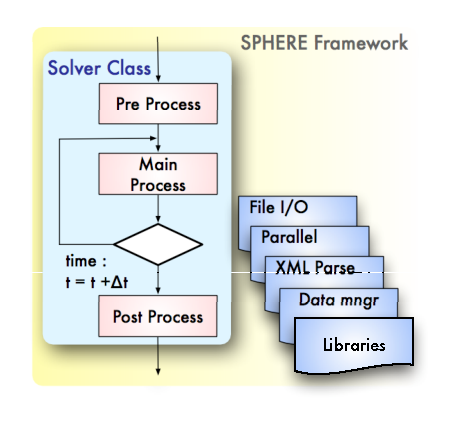
\includegraphics[width=8cm,clip]{Sphere_Control.eps}
  	\end{center}
  	\caption{V-Sphereの制御構造.プリ,メイン,ポストの処理プロセスが組み込まれており,提供されるライブラリ機能を用いてソルバークラスを構築する.}
	\label{fig:Control_structure}
  \end{minipage} \hfill
  \begin{minipage}{.47\textwidth}
	\begin{center}
  	\includegraphics[width=7.5cm,clip]{CubeFamilies.eps}
  	\end{center}
  	\caption{差分プログラミングによるソルバークラスの開発.SklSolverBaseクラスから派生させて目的のソルバークラスを作成する.ソルバークラスC3D-AはC3Dから派生しており,必要な機能だけが追加でプログラミングされる.また,必要に応じて,ユーザが定義したクラスライブラリに共通機能をまとめて利用できる.}
  	\label{fig:DerivedSolvers}
  \end{minipage}
  \vspace*{2mm}
\end{figure}

V-Sphereは,非定常物理シミュレーションのソルバー開発を支援する抽象度の高い汎用的なプログラム部品群をクラスライブラリの形式で提供する.
それらのうち主要なクラスはSklSolverBaseクラスに既に組み込まれている.
例えば,ファイル入出力,ソルバー制御・物理・境界条件パラメータの読み込みと保持,ボクセルデータの前処理,境界条件の制御などの機能があり,プログラムに対するユーザーインターフェイスを規定する役割を果たす.

V-Sphereの機能を用いて作成したアプリケーションはソルバークラスとしてV-Sphere自身に登録することができ,登録されたソルバークラス群は共通のユーザインターフェイスを備えたアプリケーションとして振る舞う.これはエンドユーザから見ると,利用しやすいアプリケーション群と認識されるであろう.
V-Sphere では,\textbf{図\ref{fig:DerivedSolvers}}に示すようにSklクラス,SklBase\index{SklBase}クラス,およびSklSolverBaseクラスを提供する.SklSolverBaseクラスからSklSolverFBクラスとSklSolverStructクラスが派生し,さらにSklSolverFBクラスからは各ソルバクラスが派生している.
\textbf{図\ref{fig:DerivedSolvers}}には,ソルバークラスC3Dから派生した2つのソルバークラスを示している.
これらの2つのソルバークラスC3D-A, C3D-Bは,基本的な機能はC3Dクラスの機能を持つが,例えば,シミュレートする物理現象や形状近似度,変数配置などが異なるソルバーと考えることができる.
異なるソルバーであっても,同じ基底クラスを利用してアプリケーションを開発することによって,ユーザーインターフェイスが統一されたアプリケーションとして構築することができる.

具体的なアプリケーションを構築する場合には,V-Sphereが提供する基本的な機能部品を用いて,より具体的な機能を構成する必要がある.
つまり,ソルバークラスの詳細な処理の記述はユーザに任されている.
そこで,適用範囲を限定しながらもある程度の汎用性をもつクラスを作成する必要がある.
これには,二種類の方法がある.
\textbf{図\ref{fig:V-Sphere_framework}}において,ユーザー定義クラス\index{ゆーざーていぎくらす@ユーザー定義クラス}やユーザー定義基底クラス\index{ゆーざーていぎきていくらす@ユーザー定義基底クラス}がそれに相当する.
ユーザー定義クラスは,文字通り,ユーザーが作成したクラスである.ユーザー定義クラスは通常のオブジェクト指向プログラミングに従い,SklSolverBaseクラスの中でインスタンスして利用することができる.
一方,ユーザー定義基底クラスは,SklSolverBaseクラスを派生させたクラスで,これからさらに派生させたソルバークラスでの利用を想定している.
つまり,ソルバー開発者はユーザー定義基底クラスを派生させて具体的なソルバークラスを作成する.
V-Sphereを用いたコード開発では,両方のアプローチを利用している.

シミュレーションプログラムの利用価値を高めるためには,コードのポータビリティを始めとして,開発の効率化支援と共にメンテナンス性や利用環境なども考慮する必要がある.
この観点から,V-Sphereは開発者とエンドユーザーの双方に利便性を提供する.

\begin{itemize}
\item 開発の効率化\\
フレームワークの利用により,上位概念でプログラミングができる.つまり,アプリケーション開発者はアルゴリズムの記述に専念でき,またプログラムのメンテナンスが簡単になる.
他方,デメリットとしてはソルバー開発者に,プログラム・データ構造やコーディングの作法を強制する面がある.
\item エンドユーザーに対するインターフェイスの統一化\\
利用するソルバーが異なってもアプリケーションの振る舞いは同様であるので,アプリケーション導入時のハードルは低くなる.
\end{itemize}

大規模な解析を実施する観点からは,並列化が必須となってくる.
V-Sphereは,並列化も含めシミュレーションプログラム開発の効率的な開発環境を提供すること,マルチフィジックス問題を扱うことも視野に入れ複数のコードの実行管理を行うことを視野に入れている.
逐次コードから並列コードへの拡張については,簡単なライブラリコールにより領域分割型の並列化に対応できるように工夫され,高い並列化性能がでることを確認している.

%
\section{ソルバークラス}
\label{sec:1.2}
V-Sphereに移植されたソルバークラスを\textbf{表\ref{tbl:solverclass}}に示す\footnote{\today 現在}.FBクラスは,具体的な流体ソルバークラスを開発するために使うクラス群であり,単体では動作しない.

\begin{table}[htdp]
\caption{V-Sphereで稼働するソルバークラス}
\small
\begin{center}
\begin{tabular}{ll} \toprule
Solver Class & Solverの説明\\ \midrule
CBC & 直交系の単層流三次元非圧縮非定ソルバークラス\\
FB & 流体解析に用いる基本パッケージクラス\\ \bottomrule
\end{tabular}
\end{center}
\label{tbl:solverclass}
\end{table}

%
\section{V-Sphereユーザーガイドの構成}
\label{sec:1.3}
本ユーザーガイドの構成は以下のようになっている.2章ではMPI通信ライブラリ,V-Sphereの環境設定,およびソルバークラスのインストールについて詳細に記述している.



%%%
\chapter{並列ライブラリ}
\begin{abstract}
MPI通信ライブラリ\index{えむぴーあいつうしんらいぶらり@MPI通信ライブラリ}のインストール概要について説明する.
MPI通信ライブラリは,mpich1\index{mpich}~\cite{mpich1}, mpich2\index{mpich2}~\cite{mpich2}, OpenMPI\index{OpenMPI}~\cite{openmpi}など,いずれでも良い.
本章ではmich1, mpich2, OpenMPIについてインストール方法を記す.
\end{abstract}
%

%
\section{mpich1}
\label{sec:mpich1}

\begin{enumerate}

\item 簡単な手順\footnote{Macの場合には,-rsh=ssh を使用する.Intel Compiler C/C++ 10.1では,multibyteの文字コードの対応が不充分のようで、デフォルトの設定ではうまく動かない.
このため,configure時には次のオプションをつける.version 11.0, rev.056以降では,-no-multibyte-charsは不要.\\
"-cflags='-O3 -no-multibyte-chars' -c++flags='-O3 -no-multibyte-chars'"
}

\begin{indentation}{3zw}{0zw}
Intel Mac, Intel Compiler 11.1の場合について示す.

{\small
\begin{program}
$ ./configure --prefix=/usr/local/mpich -cc=icc -c++=icpc -fc=ifort -f90=ifort \
              -cflags=-O3 -c++flags=-O3 -rsh=ssh
$ make
$ sudo make install
\end{program}
}
\end{indentation}
\vspace{3mm}

\item トラブルシューティング\index{トラブルシューティング}\\
\begin{indentation}{3zw}{0zw}

\begin{itemize}
\item gcc でもiccでも可能.
configure時に環境変数を使う指示があるが,このconfigure はコマンドラインで指定すること.
\footnote{Intel Compiler C/C++ ver.10までは,32ビット用コンパイラと64ビット用コンパイラが混在している.Intel64のプラットホームで,cc(32bit), cce(64bit) の両方がある場合,先にcceを記述する.\\
"PATH=/usr/local/mpich/bin:/opt/intel/cce/10.1/bin:/opt/intel/cc/10.1/bin"
}

{\small
\begin{program}
--prefix=/usr/local/mpich
-fc=ifort
-f90=ifort
-rsh=rsh or ssh
\end{program}
}
\vspace{3mm}

\item fortranの設定ができていない場合には, /usr/local/mpich/bin配下にmpif90などのインクルードファイル,include配下にmpif.h, f90choice/などができていないので,この点を確認する.
configureの内容は,bin/mpireconfig.datの先頭付近にコメントとして書かれている.両方を試す場合には,
{\small
\begin{program}
/usr/local/mpich.gcc
/usr/local/mpich.intel
\end{program}
}
などをつくり,/usr/local/mpich にスタティックリンクを張る.
{\small
\begin{program}
$ cd /usr/local
$ sudo ln -s mpich.intel/ mpich
\end{program}
}
\vspace{3mm}

\item システムの設定で,場合によっては/usr/bin/mpirun\index{mpirun}がコールされる場合がある.
これはPATHで/usr/local/mpich/binを先に見るように設定しておく.
\vspace{3mm}

\item sphereのコンパイルで,libxml2のpthread関連のエラーが出ることがある.
make.IA64\_linuxなどで,XMLLIBSの最後に-lpthreadを追加して対応する.
\vspace{3mm}

\item リンクエラーが出た場合,
{\small
\begin{program}
$ nm *.a | less
\end{program}
}
などで,該当の関数を探す.
記号Tを全て探して,対象のアーカイブをリンクするようにmake.*を変更する.
具体的には,FCLIBS=...
\vspace{3mm}

\item LinuxでIntel Compiler 10.x/11.xの場合,
{\small
\begin{program}
-cflags='-O3 -no-multibyte-chars' -c++flags='-O3 -no-multibyte-chars'
\end{program}
}
\vspace{3mm}

\item Intel mac OSX 10.5で,Intel Compiler 11.0/11.1の場合,rshは必ずsshのこと.また,Intel Compiler 10.1の場合には,Linuxの場合と同様に"-no-multibyte-chars"が必要.
{\small
\begin{program}
$ ./configure --prefix=/usr/local/mpich -cc=icc -c++=icpc -fc=ifort -f90=ifort \
              -cflags=-O3 -c++flags=-O3 -rsh=ssh
\end{program}
}
\vspace{3mm}

\end{itemize}
\end{indentation}

\end{enumerate}

%%%%%%%
\begin{comment}
\section{mpich2}
\label{sec:mpich2}

\begin{enumerate}

\item コンパイル環境の設定\footnote{Windows IA32\index{Windows}においてmpich2をインストールするためには,
「Microsoft Visual Studio 2008」\index{Visual Studio}\\
あるいは,\\
「Microsoft Visual C++ (2005または)2008 SPI 再頒布可能パッケージ(x86)」\\
「Windows Installer 3.1 Redistributable(v2) - 日本語」\\
「Microsoft .NET Framework 3.5」\\
の3点を前もってインストールすることが必要.詳細は,V-SphereのWindowsマニュアルを参照のこと.}

\begin{itemize}
\item /usr/local/mpich2にインストールし,/usr/local/mpichにリンクする
\item ”ssm”(sockets and shared memory) クラスタ間のプロセス間通信はソケット通信,SMP上のプロセス間通信は共有メモリを利用するデバイスとチャネルを選択する.\footnote{mpich2では,特定のチャネルと対になったデバイスにより通信が行われる.デフォルトでは,ch3デバイス上のsockチャネルが設定される.ch3デバイス上のチャネルは他にも,nemesis, shm(shared memory), ssm(sockets and shared memory) がある.ssmでは,マルチスレッドは現時点でのサポートなし.MPI\_THREAD\_MULTIPLEは,sockとnemesisのみ.現リリース(mpich2-1.0.7-rc1)では,デフォルトチャネル(sock)以外を利用する場合,環境変数にチャネル名をセットすること.\\
\verb|$ export MPICH_CH3CHANNEL=SSM|
}
\item 共有ライブラリを利用(コンパイラはgccのみに対応)
\item 環境変数のセット(インストール時にテンポラリに)\footnote{共有メモリオプションを利用する場合には,gccのサポートしかないので,gcc を利用する.}
\end{itemize}
\vspace{\baselineskip}

\item 簡単な手順
\begin{indentation}{3zw}{0zw}
{\small
\begin{verbatim}
$ export CC=gcc4
$ export CFLAGS=’-O3 -m64’
$ export CXX=g++
$ export CXXFLAGS=’-O3 -m64’
$ export F77=ifort
$ export FFLAGS=’-O3’
$ export F90=ifort
$ export F90FLAGS=’-O3’
$ export MPICH_CH3CHANNEL=SSM
$ export MPICH_DEVICE=’--with-device=ch3:ssm’

$ ./configure --prefix=/usr/local/mpich2
              --enable-error-checking=no
              --enable-error-messages=none
              --enable-timing=none
              --enable-g=none
              --enable-fast
              --enable-ndebug
              --enable-f77
              --enable-f90
              --enable-cxx
              --enable-romio
              --enable-threads=single
              --with-thread-package=posix
\end{verbatim}
\verb|              --enable-sharedlibs=gcc|\footnote{Mac OSXの場合は\quad \verb|--enable-sharedlibs=osx-gcc|
}

\begin{verbatim}
$ make
$ sudo make install

$ cd /usr/local
$ sudo ln -s mpich2 mpich
\end{verbatim}
}
\end{indentation}
\vspace{\baselineskip}

\item トラブルシューティング
{\small
\begin{itemize}
\item Windows\index{Windows}でSP3をインストールしてある場合\\
Windows Installer 3.1 Redistibutable(v2)-日本語をインストールする場合に,「このシステムのService Packが適用しようとしている更新より新しいバージョンであることが検出されました。この更新をインストールする必要はありません」とメッセージがでて,インストールされていないかもしれないがインストール自体は完了している.
\vspace{\baselineskip}
\item gccのエラー\\
\verb|$ export CC=gcc4|\quad では、C compilerが見つからないというエラーが出る場合がある.
\begin{verbatim}
checking for gcc... gcc4
checking for C compiler default output file name...
configure: error: C compiler cannot create executables
\end{verbatim}
この場合,gccを用いる.
\vspace{\baselineskip}
\end{itemize}

}
\end{enumerate}
\end{comment}
%%%%%%%

\section{mpich2}
\label{sec:mpich2}
mpich2を例に説明する.

%
\begin{enumerate}
\item 簡単な手順\\
MPICH2のWEBサイト\footnote{\url{http://www.mcs.anl.gov/research/projects/mpich2/}\\
2011年5月12日現在,安定リリース版はmpich2-1.3.2p1.tar.gzである.}から,ソースをダウンロードして解凍する.

作成されたディレクトリに入り,configureのために,次のようなスクリプトを用意し,実行する.
インストールディレクトリは,/usr/local/mpich2とする.

%
\begin{indentation}{3zw}{0zw}
{\small
\begin{program}
$ cat config_mpich2.sh
-----------------------------------
#!/bin/sh
export CC=icc
export CFLAGS=-O3
export CXX=icpc
export CXXFLAGS=-O3
export F77=ifort
export FFLAGS=-O3
export FC=ifort
export FCFLAGS=-O3
#
./configure --prefix=$1
-----------------------------------

$ ./config_mpich2.sh /usr/local/mpich2

$ make

$ sudo make install
\end{program}
}
\end{indentation}

\end{enumerate}


%%%
\section{OpenMPI}
\label{sec:ompi}
OpenMPI-1.3.2を例に説明する.

%
\begin{enumerate}
\item 簡単な手順\\
configureのために,次のようなスクリプトを用意し,実行する.インストールディレクトリは/usr/local/ompiとする.

\begin{indentation}{3zw}{0zw}
{\small
\begin{program}
$ cat config_ompi.sh
------------------------------
#!/bin/sh
export CC=icc
export CFLAGS=-O3
export CXX=icpc
export CXXFLAGS=-O3
export F77=ifort
export FFLAGS=-O3
export FC=ifort
export FCFLAGS=-O3
#
./configure --prefix=$1 
------------------------------

$ ./config_ompi.sh /usr/local/ompi

$ make

$ sudo make install
\end{program}
}
\end{indentation}
\vspace{\baselineskip}

\item PATHの設定\\
実行時のmpiexec\footnote{mpirunでも動く.}が正しいパスになっているかどうかをwhichコマンドで確認する.
\begin{indentation}{3zw}{0zw}
{\small
\begin{program}
$ which mpiexec
/usr/bin/mpiexec
\end{program}
}
\end{indentation}

Mac OSXの場合には上記のように,デフォルトでインストールされているOpenMPIの方を見に行くので,インストールしたOpenMPIのPATHを最初の方に書いておく.
\begin{indentation}{3zw}{0zw}
{\small
\begin{program}
$ cat .bash_priofile

#! /bin/sh
PATH=~/bin:~/bin/script:/usr/local/ompi/bin:${PATH}; export PATH
...
. ~/.bashrc

\end{program}
}
\end{indentation}

\end{enumerate}





%%%
\chapter{V-Sphere}
\begin{abstract}
この章では,V-Sphereのインストール概要について説明する.
\end{abstract}
%

%
\section{インストール}
\label{sec:install}
V-Sphereのインストールは,MPI通信ライブラリのインストールが終了したあとに行う.
V-Sphereは,単精度版と倍精度版を別々に用意する必要がある.

\begin{enumerate}

\item configure\footnote{ここでは,MacOSX,IA-64モード,コンパイラの環境として,/opt/intel/Compiler/11.1/089のディレクトリを仮定,コンパイルオプション\index{コンパイルオプション}として,-O3 を指定.icc, icpc, ifortへのパスは既に指定していると仮定する.特別な仕様のマシン向けのインストールには,makefile.specを使う.これは,特別な仕様のマシン向け(p4-dev)である.\hyperlink{tgt:BGL}{BlueGene/L}の項やV-Sphereのマニュアルを参照のこと.アーキテクチャに相応しいコンパイルオプションがわからない場合は,「CXXFLAGS=-O3」「F90FLAGS=-O3」だけでも可.Intel Compiler C/C++ version 10は,multibyteの文字コードの対応が不充分のため,C/C++のコンパイルオプションで-no-multibyte-charsを明示的に指示する.Mac用のIntel Compiler 11.0では不要だが,Linuxでは必要.
}

\paragraph{コマンドライン}
コマンドラインで作業する場合には,次のようにタイプする.インストールディレクトリには\verb|/usr/local/sphere/|を指定している.もし,\verb|/usr/local/|領域へのアクセス権限がない場合には,各ユーザが書き込めるところを指定する.また,LDFLAGSには適切なパスを指定する.

{\small
\begin{program}
$ ./configure --prefix=/usr/local/sphere \
              --with-comp=INTEL \
              --with-ompi=/opt/openmpi  \
              CC=icc \
              CFLAGS='-O3'\
              CXX=icpc \
              CXXFLAGS='-O3'\
              FC=ifort \
              FCFLAGS='-O3'\
              F90=ifort \
              F90FLAGS='-O3'\
              LDFLAGS=-L/opt/intel/Compiler/11.1/089/lib
\end{program}
}

configureでインストール先を指定すると,指定したインストールディレクトリはソースディレクトリの\verb|sphconfig/sph-cfg.xml|に記録される.このファイルは,インストールディレクトリの\verb|config/sph-cfg.xml|にコピーされ,sphPrjToolのresetコマンドで参照される.このため,一旦インストールディレクトリを指定したら,移動したりリネームすると,resetコマンドが正しく機能しなくなるので注意する.

%
\paragraph{倍精度モジュール}
倍精度計算をする場合には,V-Sphereは倍精度モジュールとしてコンパイルする必要がある.configure時のオプションに\verb|--with-real=double|を追加する.このオプションにより,C/C++コンパイラに\verb|-DREAL_IS_DOUBLE|,Fortranコンパイラには\verb|-r8|がコンパイルオプションとして自動的に追加される.

\paragraph{シェル}
次のインストールシェルは,引数としてインストールディレクトリを指定する.

{\small
\begin{program}
$ configure.sh /usr/local/sphere
\end{program}
}

{\small
\begin{program}
------------------------------------
configure.sh (mpich + float)
------------------------------------
#! /bin/sh
./configure --prefix=$1 \
            --with-comp=INTEL \
            --with-mpich=/usr/local/mpich \
            CC=icc \
            CFLAGS=-O3\
            CXX=icpc \
            CXXFLAGS=-O3\
            FC=ifort \
            FCFLAGS=-O3\
            F90=ifort \
            F90FLAGS=-O3\
            LDFLAGS=-L/opt/intel/Compiler/11.0/059/lib

------------------------------------
configure.sh (mpich + double)
------------------------------------
#! /bin/sh
./configure --prefix=$1 \
            --with-comp=INTEL \
            --with-real=double \
            --with-mpich=/usr/local/mpich \
            CC=icc \
            CFLAGS=-O3\
            CXX=icpc \
            CXXFLAGS=-O3\
            FC=ifort \
            FCFLAGS=-O3\
            F90=ifort \
            F90FLAGS=-O3\
            LDFLAGS=-L/opt/intel/Compiler/11.0/059/lib

------------------------------------
configure.sh (OpenMPI + float)
------------------------------------
#! /bin/sh
./configure --prefix=$1 \
            --with-comp=INTEL \
            --with-ompi=/usr/local/ompi \
            CC=icc \
            CFLAGS=-O3\
            CXX=icpc \
            CXXFLAGS=-O3\
            FC=ifort \
            FCFLAGS=-O3\
            F90=ifort \
            F90FLAGS=-O3\
            LDFLAGS=-L/opt/intel/Compiler/11.0/059/lib

------------------------------------
configure.sh (OpenMPI + double)
------------------------------------
#! /bin/sh
./configure --prefix=$1 \
            --with-comp=INTEL \
            --with-real=double \
            --with-ompi=/usr/local/ompi \
            CC=icc \
            CFLAGS=-O3\
            CXX=icpc \
            CXXFLAGS=-O3\
            FC=ifort \
            FCFLAGS=-O3\
            F90=ifort \
            F90FLAGS=-O3\
            LDFLAGS=-L/opt/intel/Compiler/11.0/059/lib
\end{program}
}


\item make
\footnote{make時にlibimf.soが見つからないなどのメッセージが出る場合は,ユーザのLD\_LIBRARY\_PATHにパス を加えておく.\\
"LD\_LIBRARY\_PATH=/opt/intel/Compiler/11.0/056/lib:/usr/local/mpich/lib"}

{\small
\begin{program}
$ make
\end{program}
}
\vspace{\baselineskip}

\item Install
{\small
\begin{program}
$ sudo make install または make install
\end{program}
}

V-Sphereライブラリがインストールディレクトリにインストールされると,次に示すようなコンパイルに関する情報がソースディレクトリの\verb|sphconfig/sph-cfg.xml|に記述される.
{\small
\begin{program}
<SphereEnvironment>
  <Param name="SPHEREDIR" dtype="STRING" value= "/usr/local/sphere"/>
  <Param name="CXX" dtype="STRING" value="icpc"/>
  <Param name="CXXFLAGS" dtype="STRING" value="-O3"/>
  <Param name="CC" dtype="STRING" value="icc"/>
  <Param name="CFLAGS" dtype="STRING" value="-O3"/>
  <Param name="FC" dtype="STRING" value="ifort"/>
  <Param name="FCFLAGS" dtype="STRING" value="-O3"/>
  <Param name="F90" dtype="STRING" value="ifort"/>
  <Param name="F90FLAGS" dtype="STRING" value="-O3"/>
  <Param name="LDFLAGS" dtype="STRING" value="-L/opt/intel/Compiler/11.1/067/lib"/>
  <Param name="SPH_DEVICE" dtype="STRING" value="Snow_Leopard"/>
  <Param name="MPICH_DIR" dtype="STRING" value="/usr/local/ompi"/>
  <Param name="MPICH_CFLAGS" dtype="STRING" value="-I/usr/local/ompi/include"/>
  <Param name="MPICH_LDFLAGS" dtype="STRING" value="-L/usr/local/ompi/lib"/>
  <Param name="MPICH_LIBS" dtype="STRING" value="-lmpi"/>
  <Param name="XML2FLAGS" dtype="STRING" value="-I/usr/include/libxml2"/>
  <Param name="XML2LIBS" dtype="STRING" value="-lxml2 -lz -lpthread -licucore -lm"/>
  <Param name="SPHERE_CFLAGS" dtype="STRING" value="-DSKL_TIME_MEASURED -D_CATCH_BAD_ALLOC 
               -I/usr/local/vsph175/include"/>
  <Param name="SPHERE_LDFLAGS" dtype="STRING" value="-L/usr/local/vsph175/lib"/>
  <Param name="SPHERE_LIBS" dtype="STRING" value="-lsphapp -lsphbase -lsphls -lsphfio -lsphdc 
               -lsphcrd -lsphcfg -lsphftt -lsphvcar"/>
  <Param name="LIBS" dtype="STRING" value="-lifport -lifcore"/>
</SphereEnvironment>
\end{program} 
}

%
\paragraph{マニュアルインストール}
別の方法として,Config.specを編集する.
ポイントは,libxml2とinstallコマンドのパス.
{\small
\begin{program}
$ xml2-config --libs
\end{program}
}
を実行してメッセージが返ればOK.
{\small
\begin{program}
$ which install
\end{program}
}
インストールコマンドがあればOK.
その後,
{\small
\begin{program}
$ make -f Makefile.spec
# make -f Makefile.spec install
\end{program}
}
\vspace{\baselineskip}

\item インストールに失敗する場合\\
makeに失敗して,何度もインストールしているとMakeで使用する環境変数がおかしくなることがある.
やり直すときは、コンフィギュレーションをクリアし,最初からインストール作業を行う.

{\small
\begin{program}
$ make distclean  (コンフィギュレーションのクリア)
\end{program}
}

ただし,再インストールの場合はtarボールから解凍して再試行する方がより安全.
また,上記の\verb|make distclean|を実行すると,設定ファイルが全て消去される.

\end{enumerate}

%%
\section{アンインストール}
V-Sphereをアンインストール\index{アンインストール!V-Sphereの@V-Sphereの---}する場合には,インストールしたディレクトリ(configureでオプション指定したディレクトリ)のsphereを削除する.


%
\chapter{プロジェクトツールを用いた開発環境の構築}
\begin{abstract}
この章では,ソルバークラスの開発を行うために,プロジェクトツールを用いた環境構築について説明する.
ソルバーの開発を行わない,エンドユーザは本章は読み飛ばして構わない.
\end{abstract}
%

%
\section{sphPrjToolを用いた開発環境の構築}

本節では,V-Sphereを用いた開発を行う場合の環境を設定する.ツールとして,sphPrjTool\index{sphPrjTool}を用いる.sphPrjToolの詳細については,V-Sphereのマニュアル04\_UtilityToolsを参照のこと.
また,PRJ\_CBCが提供されている場合は,「CBC\_UG.pdf」の「2.3.2 sphPrjToolを用いた簡単なインストール」を参照のこと.

%
\subsection{sphPrjTool}
\label{sec:sphPrjTool}

例として,CBCソルバークラスについて説明する.
以下のようなソースツリーを想定する.

\begin{indentation}{3zw}{0zw}
\small
\begin{program}
CBC-x.x.x
  |
  +- src                          ソースコード
      +- project_local_settings   プロジェクトのコンパイル環境設定
      +  F_CBC                    CBCクラスのFortranファイル
      +- F_CPC                    CPCクラスのFortranファイル
      +- F_VOF                    VOFクラスのFortranファイル
      +- FB                       FlowBaseクラス(ユーザー定義クラス群)
      +- IP                       組み込み例題クラス群
\end{program}
\end{indentation}
\vspace{\baselineskip}

%
\subsubsection{プロジェクトの作成とソースファイルの登録}
まず,src直下のディレクトリでsphPrjToolを起動し,プロジェクト名とソルバーキーワードを登録,登録内容を確認してセーブする.
{\small
\begin{program}
$ cd src 
$ sphPrjTool
sphPrjTool> help
sphPrjTool> new -p PRJ_CBC
sphPrjTool> new -s CBC
sphPrjTool> print
sphPrjTool> save
sphPrjTool> quit
\end{program}
}

\noindent 以下に,printの出力結果を示す.

{\small
\begin{program}
sphPrjTool> print         
Project Name : PRJ_CBC
  Compile Environment
    CC                  : icc
    CFLAGS              : -O3
    CXX                 : icpc
    CXXFLAGS            : -O3
    FC                  : ifort
    FCFLAGS             : -O3
    F90                 : ifort
    F90FLAGS            : -O3
    LDFLAGS             : -L/opt/intel/composerxe/lib
    LIBS                : -lifport -lifcore
    SPH_USR_DEF_LIBS    : 
    UDEF_OPT            : -DTD_USE_NAMESPACE -DNON_POLYLIB -DNON_CUTLIB
    UDEF_INC_PATH       : -I../../Cutlib_2_0_0/include -I../../Polylib_2_0_2/include
    UDEF_LIB_PATH       : -L../../Polylib_2_0_2/lib -L../../Cutlib_2_0_0/lib
    UDEF_LIB_UPPER      : 
    UDEF_LIB_LOWER      : 
    Use Module.
        Generate parallel module.

    ---
    Reference only (Unmodifiable):
    SPHEREDIR           : /usr/local/sphere
    SPH_DEVICE          : Snow_Leopard
    MPICH_DIR           : /opt/openmpi
    MPICH_CFLAGS        : -I/opt/openmpi/include
    MPICH_LDFLAGS       : -L/opt/openmpi/lib
    MPICH_LIBS          : -lmpi
    XML2FLAGS           : -I/opt/local/include/libxml2
    XML2LIBS            : -L/opt/local/lib -lxml2 -lz -lpthread -liconv -lm
    SPHERE_CFLAGS       : -DSKL_TIME_MEASURED -D_CATCH_BAD_ALLOC -I/usr/local/vsph184_float_64/include
    SPHERE_LDFLAGS      : -L/usr/local/vsph184_float_64/lib
    SPHERE_LIBS         : -lsphapp -lsphbase -lsphls -lsphfio -lsphdc -lsphcrd -lsphcfg 
                          -lsphftt -lsphvcar
    SKL_REAL is float. (REALOPT = float)
    ---

  Regist Solver
    Name : CBC
      Regist file :
        FortranFuncCBC.h
        SklSolverCBCDefine.h
        SklSolverCBCInitialize.C
        SklSolverCBCLoop.C
        SklSolverCBCPost.C
        SklSolverCBCUsage.C
        SklSolverCBC.C
        SklSolverCBC.h
\end{program}
}

\noindent この作業で,作業ディレクトリでは以下のようなファイル構成になる.

{\small
\begin{program}
PRJ_CBC/
   |
   +app/Makefile
   |    SklCreateSolver.C
   |    SklDeleteSolver.C
   |    SklFactoryCBC.C
   |    SklFactoryCBC.h
   |    SklSolverType.h
   |
   +bin/
   |
   +CBC/CBC.xml
   |    FortranFuncCBC.h
   |    Makefile
   |    SklSolverCBC.C
   |    SklSolverCBC.h
   |    SklSolverCBCDefine.h
   |    SklSolverCBCInitialize.C
   |    SklSolverCBCLoop.C
   |    SklSolverCBCPost.C
   |    SklSolverCBCUsage.C
   |
   Makefile
   PRJ_CBC.xml               プロジェクト設定ファイル
   project_local_settings    コンパイル時に利用する環境設定ファイル
   
\end{program}
}

\noindent 次に,プロジェクト設定ファイルを指定して起動する.
{\small
\begin{program}
$ cd PRJ_CBC
$ sphPrjTool PRJ_CBC.xml  
\end{program}
}
\noindent または,sphPrjTool\index{sphPrjTool}起動後に\\

{\small
\noindent \verb|> load PRJ_CBC.xml|\\
\\
}
\noindent とすると,ファイルの登録や環境設定が行える.詳細は,マニュアルおよびヘルプコマンドを参照のこと.
新規にソースファイルをSOLVER\_NAMEにリンクする場合には,下記の操作を行う.
ファイル名は必ず絶対パスか,sphPrjToolを起動したディレクトリからの相対パスを指定する.内部的には,プロジェクトディレクトリ\footnote{プロジェクト情報が格納されるディレクトリ.つまり,プロジェクトのコンフィギュレーションファイル(プロジェクト名.xml)の存在するディレクトリ.}を基点として相対パスで記述される.
\footnote{.[Ch]は接尾辞Cまたはhをもつファイルをプロジェクトにリンクし,.f90は接尾辞f90をもつファイルをプロジェクトにリンクすることを意味する.}
{\small
\begin{program}
sphPrjTool> regist -f SOLVER_NAME *.[Ch]
sphPrjTool> regist -f SOLVER_NAME *.f90
sphPrjTool> save
\end{program}
}
sphPrjToolを使って,プロジェクト設定ファイルを修正・保存すると,環境設定ファイルproject\_local\_settingsファイルの内容が修正内容に応じて変更される.したがって,project\_local\_settingsファイルを直接編集して環境設定を行った場合は,プロジェクト設定ファイルを修正・保存するとproject\_local\_settingsファイルの内容がリセットされてしまうので,注意すること.

%
\subsubsection{PLSファイルの設定}
project\_local\_settingsファイルは,上記の作業でPRJ\_CBCの直下に生成される.もし,複数のプロジェクトで共通の設定を利用する場合には,src直下に移動することも考えられる.その場合には,プロジェクトの設定で,次のようにproject\_local\_settingsファイルの読み込み先を変更する.

{\small
\begin{program}
$ pwd
CBC-x.x.x/src/PRJ_CBC

$ mv project_local_settings ..

$ sphPrjTool PRJ_CBC.xml  
sphPrjTool> setpls ../project_local_settings
sphPrjTool> save
sphPrjTool> quit
\end{program}
}

\noindent これにより,プロジェクト情報は次のように表示される.

{\small
\begin{program}
sphPrjTool> print
    ...
    project_local_settings="../project_local_settings". (Relative path from Prj-Dir)
    ...
\end{program}
}

%
\subsubsection{並列モジュールの指定}
並列版のソルバー実行モジュールを作成する場合には,moduleコマンドを用いて指定する.
{\small
\begin{program}
sphPrjTool> module parallel
sphPrjTool> print
    ...
    Generate parallel module.
    ...
\end{program}
}

%
\subsubsection{ユーザ定義のオプション指定}
reset localsetting コマンドでリセットされないユーザが指定オプションは環境変数で指定する.
詳細はV-Sphereマニュアルを参照.

{\small
\begin{program}
sphPrjTool> env UDEF_*
sphPrjTool> print
   ...
   UDEF_OPT=-DTD_USE_NAMESPACE -DNON_POLYLIB -DNON_CUTLIB
   UDEF_INC_PATH=-I../../Cutlib_2_0_0/include -I../../Polylib_2_0_2/include
   UDEF_LIB_PATH=-L../../Polylib_2_0_2/lib -L../../Cutlib_2_0_0/lib
   UDEF_LIB_UPPER=
   UDEF_LIB_LOWER=
   ...
\end{program}
}

%
\section{ユーザ定義の非ソルバーモジュールの導入}
\label{sec:non-solver module}

非ソルバーモジュールとして,ユーザ定義クラス\index{ゆーざていぎくらす@ユーザ定義クラス}を作成する.
ユーザ定義クラスは,ソルバークラス内で使用するユーザが作成したクラス群である.

PRJ\_CBCディレクトリでsphPrjToolを起動し,非ソルバーモジュールをプロジェクトに組み込む.複数のモジュールを利用する場合には,ライブラリのリンク順を考慮する必要があるため\footnote{Makefile 中のSPH\_SOLV\_FLAGS などの順序が重要となる.},モジュール間の依存関係による読み込む.モジュールを登録するとき,基底クラスを後で登録する点に注意する.ここでは,CBC $\gg$ IP $\gg$ FBのような依存関係がある(左のモジュールは右に依存している).

{\small
\begin{program}
$ sphPrjTool PRJ_CBC.xml
sphPrjTool> new -o IP
sphPrjTool> new -o FB
sphPrjTool> save
sphPrjTool> quit
\end{program}
}

\noindent プロジェクト情報は次のように表示される.

{\small
\begin{program}
sphPrjTool> print
  ...
  Regist NonSolver
    Name : IP
    Name : FB
\end{program}
}

次に,ソルバークラスと非ソルバーモジュールにソースファイルを登録する.
{\small
\begin{program}
$ sphPrjTool PRJ_CBC.xml  
sphPrjTool> regist -f IP ../IP/*.[Ch]
sphPrjTool> regist -f FB ../FB/*.[Ch]
\end{program}
}
\noindent または,FB.xmlファイルなどを直接編集した後,sphPrjToolで再度PRJ\_CBC.xmlファイルをロードとセーブすると変更が反映される.

\begin{indentation}{3zw}{0zw}
\small
\begin{program}
CBC-x.x.x
  |
  +- src                          ソースコード
      +- project_local_settings   プロジェクトのコンパイル環境設定
      +  F_CBC                    CBCクラスのFortranファイル
      +- F_CPC                    CPCクラスのFortranファイル
      +- F_VOF                    VOFクラスのFortranファイル
      +- FB                       FlowBaseクラス(ユーザー定義クラス群)
      +- IP                       組み込み例題クラス群
      |
      +- PRJ_CBC	                 CBCプロジェクト
         +- app                  アプリケーションコンパイルディレクトリ
         +- bin                  バイナリモジュール格納ディレクトリ
         |
         +- CBC                  CBCソルバークラスのソースファイル
         |   +- CBC.xml          CBCクラスのコンパイル環境設定
         |
         +- FB                   非ソルバークラスディレクトリ FlowBase
         |   +- FB.xml           FBクラスのコンパイル環境設定  
         |
         +- IP                   非ソルバークラスディレクトリ 組み込み例題クラス群
         |   +- IP.xml           IPクラスのコンパイル環境設定 
         |
         +- Makefile             アプリケーションコンパイル用 Linux/Mac
            PRJ_CBC.xml          CBCのコンパイル設定

\end{program}
\end{indentation}


%%%%%%
\begin{comment}
\subsection{ユーザ定義の基底クラスの導入}
本節では,ユーザ定義基底クラス\index{ゆーざていぎきていくらす@ユーザ定義基底クラス}を用いたソルバーの構築方法について記述する\footnote{本節の内容は古いので,作業については確認のこと}.
UDBCをユーザが定義した基底クラスとし,CBS3D\_ICクラスがUDBCクラスを継承しているとする.
UDBCクラスの雛型は,別のディレクトリに保存しておき,sphPrjTool\index{sphPrjTool}で PROJECT\_NAME/UDBC を作成後にファイルをコピーする.
\footnote{派生クラスのプロジェクトを作成するときの注意点\\ プロジェクトにソルバクラスを登録するとき,基底クラスを後で登録すること.
これは,ライブラリのリンク順に影響するため.Makefile 中のSPH\_SOLV\_FLAGS などの順序が重要となる.}\quad
UDBCクラスは,SklSolverBase\index{SklSolverBase}クラスを継承し,CBS3D\_ICクラスはSklSolverUDBC クラスを継承する.
UDBCクラスは,単体でもコンパイルは可能であるが,動作としては何もしない.\\

\subsubsection{Example}

作業ディレクトリsph\_v164を作成し,プロジェクトS4DとソルバークラスCBS3D\_ICとユーザー定義基底クラスUDBCを登録する.その後,UDBCクラスとCBS3D\_ICのファイルを登録する.\footnote{XML2LIBSのオプションは,Linuxの場合には-lconv は不要.}
{\small
\begin{program}
$ mkdir sph_v164	;ディレクトリの作成
$ cd sph_v164		
$ sphPrjTool		;プロジェクトツールの起動

sphPrjTool> new -p S4D			;プロジェクトの作成
sphPrjTool> new -s CBS3D_IC		;登録順に注意
sphPrjTool> new -s UDBC			;
sphPrjTool> print				;作業内容の確認

Project Name : S4D
  Compile Environment2
    CC                  : icc
    CFLAGS              : -O3 -axT
    CXX                 : icpc
    CXXFLAGS            : -O3 -axT
    FC                  : ifort
    FCFLAGS             : -O3 -axT
    F90                 : ifort
    F90FLAGS            : -O3 -axT
    LDFLAGS             : -L/opt/intel/fce/10.1/lib
    LIBS                : -lifport -lifcore
    XML2FLAGS           : -I/usr/include/libxml2  ;必要に応じて以下2行を検討する
    XML2LIBS            : -L/usr/lib -lxml2 -lz -lpthread -liconv -lm
    SPH_USR_DEF_LIBS    : 
    UDEF_OPT            : -DTD_USE_NAMESPACE -DNON_POLYLIB -DNON_CUTLIB
    UDEF_INC_PATH       : -I../../Cutlib_2_0_0/include -I../../Polylib_2_0_2/include
    UDEF_LIB_PATH       : -L../../Polylib_2_0_2/lib -L../../Cutlib_2_0_0/lib
    UDEF_LIB_UPPER      : 
    UDEF_LIB_LOWER      : 
    ---
    Generate non-parallel module.

  Regist Solver
    Name : CBS3D_IC
      Regist file :
        FortranFuncCBS3D_IC.h
        SklSolverCBS3D_ICDefine.h
        SklSolverCBS3D_ICInitialize.C
        SklSolverCBS3D_ICLoop.C
        SklSolverCBS3D_ICPost.C
        SklSolverCBS3D_ICUsage.C
        SklSolverCBS3D_IC.C
        SklSolverCBS3D_IC.h
    Name : UDBC
      Regist file :
        FortranFuncFB.h
        SklSolverFBDefine.h
        SklSolverFBInitialize.C
        SklSolverFBLoop.C
        SklSolverFBPost.C
        SklSolverFBUsage.C
        SklSolverFB.C
        SklSolverFB.h

sphPrjTool> save		;ディスクに内容を保存
sphPrjTool> quit		;終了
\end{program}
}
\begin{enumerate}
\item 前述の操作で,CBS3D\_IC, UDBCには,それぞれ雛型のファイルが生成される.
\item UDBCクラスのオリジナルファイルは,別ディレクトリに保存されていると仮定する.オリジナルファイルを全て上書きでコピーする.
\item CBS3D\_ICクラスのオリジナルファイルは,別ディレクトリに保存されていると仮定する.オリジナルファイルを全て上書きでコピーする.
\item 確認
{\small
\begin{program}
$ cd S4D				;作業ディレクトリの変更
$ sphPrjTool S4D.xml	;設定を読み込んで起動

sphPrjTool> print

Project Name : S4D
  Compile Environment
    CC                  : icc
    CFLAGS              : -O3 -axT
    CXX                 : icpc
    CXXFLAGS            : -O3 -axT
    FC                  : ifort
    FCFLAGS             : -O3 -axT
    F90                 : ifort
    F90FLAGS            : -O3 -xT
    LDFLAGS             : -L/opt/intel/fce/10.1/lib
    LIBS                : -lifport -lifcore
    SPH_USR_DEF_LIBS    : 
    ---
    Generate non-parallel module.

  Regist Solver
    Name : CBS3D_IC
      Regist file :
        BasketIPaxis.h
        CubeBin3D.C
        ...
        ...

    Name : FB
      Regist file :
        Basket.h
        BinaryVox.C
        BinaryVox.h
        BndOuter.h
        ...
        ...

sphPrjTool> quit
\end{program}
}
\item コンパイル時のヘッダ情報の参照のため,S4D.xmlの環境変数にインクルードパスを追加する.
{\small
\begin{program}
<Param name="CXXFLAGS" dtype="STRING" value="-O3 -axT -I../UDBC -I../CBS3D_IC"/>

$ sphPrjTool S4D.xml
sphPrjTool> print
sphPrjTool> save
sphPrjTool> quit
\end{program}
}
または,
{\small
\begin{program}
$ sphPrjTool S4D.xml
sphPrjTool> env CXXFLAGS “-O3 -axT -I../UDBC -I../CBS3D_IC”
\end{program}
}
以上で,S4Dディレクトリでmakeが可能になり,コンパイルに成功すると,S4D/bin/ 配下に実行モジュールsphereが生成される.
さらに,HCUBEクラスを組み込むと以下のようになる.\footnote{S4D.xmlを編集して,新しいソルバクラスを追加する場合には,FBクラスからの派生クラスはその前に登録しなければならない点に注意する.}
{\small
\begin{program}
$ sphPrjTool S4D.xml
sphPrjTool> new -s HCUBE
sphPrjTool> print
sphPrjTool> save
sphPrjTool> quit
\end{program}
}
S4D.xmlは下記のようになる.
{\small
\begin{program}
<Elem name="SolverClass">
  <Elem name="CBS3D_IC">
  </Elem>
  <Elem name="UDBC">
  </Elem>
  <Elem name="HCUBE">
  </Elem>
</Elem>
\end{program}
}
HCUBEとFBの順番を入れ替え,sphPrjTool\index{sphPrjTool}で読み込み保存し直す.
{\small
\begin{program}
<Elem name="SolverClass">
  <Elem name="CBS3D_IC">
  </Elem>
  <Elem name="HCUBE">
  </Elem>
  <Elem name="UDBC">
  </Elem>
</Elem>
\end{program}
}
HCUBEにファイルをコピーする.
	S4D.xmlファイルのCXXFLAGSに,-I../HCUBE を追加する.
	sphPrjToolでS4D.xmlを読み込んでから保存する.
{\small
\begin{program}
$ cd S4D
$ make allclean
$ make
\end{program}
}
以上の操作により,ディレクトリ構成は下記のようになる.
{\small
\begin{program}
TARGET_PROJECT -/Makefile
		 project_local_setting
		 TARGET_PROJECT.xml
		 Makefile
		|
		+app
		|
		+bin
		|
		+dev
		|
		+UDBC
		|
		+CBS3D_IC
		|
		+HCUBE
\end{program}
}
\end{enumerate}
\end{comment}
%%%%%%


%
\chapter{各種プラットホーム対応}
\begin{abstract}
この章では,各種プラットホームにおけるインストールについて説明する.
\end{abstract}
%

\graphicspath{{./fig5/}}

%
\section{RICC}
\label{sec:ricc}
本節では,理化学研究所のRICCシステム\footnote{http://accc.riken.go.jp/ricc.html}環境でのコンパイルについて示す.

RICCシステムでは幾種類かのコンパイラとMPIライブラリが利用可能なので,各ライブラリに合わせてコンパイルを行う.
ここでは,OpenMPIと富士通MPIについて示す.

\begin{itemize}
\item OpenMPI\\
V-Sphereのコンパイル前に,以下の修正を行う.
\begin{enumerate}
\item \verb|libmpi_cxx.so.0|のバスの設定\\
以下のコマンドを実行して,\verb|libmpi_cxx.so.0|のパスの指定を行う\footnote{後述のインストールシェルを利用する場合には,シェルに書き込んであるが,~/.bashrcに書いておくと良い.sphPrjToolの使用時にも必要.}.
{ \small
\begin{program}
$ export LD_LIBRARY_PATH=/usr/local/openmpi/intel/lib:$LD_LIBRARY_PATH
\end{program}}
\vspace{2mm}

\item \verb|CLTK_TARGET_MACHINE|の指定\\
homeディレクトリで\verb|.cltkrc|というファイルを作成し,以下の情報を記述する.
{ \small
\begin{program}
CLTK_TARGET_MACHINE = pc
\end{program}}
\vspace{2mm}

\item コンパイル\\
後述のインストールシェルを用いてインストールする.シェルの引数にはインストール先のディレクトリをフルパスで指定する.RICCではユーザは,自分の管理ディレクトリにインストールすること.
{ \small
\begin{program}
$ configure_ic_ompi.sh INSTALL_DIR
$ make
$ make install
\end{program}}
\vspace{2mm}

富士通コンパイラを利用する場合には,\verb|include/SklTiming.h|ファイルに,以下のインクルード文を追加する\footnote{V-Sphereで対応予定.}.
{ \small
\begin{program}
#include <stdio.h>
\end{program}}
\vspace{2mm}
\end{enumerate}

%
\item Fujitsu MPI\\
\begin{enumerate}
\item \verb|CLTK_TARGET_MACHINE|の指定\\
homeディレクトリで\verb|.cltkrc|というファイルを作成し,以下の情報を記述する.
{ \small
\begin{program}
CLTK_TARGET_MACHINE = pc
\end{program}}
\vspace{2mm}

\item \verb|_USE_SKL_FSEEK|の定義\\
\verb|include/endianUtil.h|ファイルに以下の記述を追加する\footnote{富士通MPIを使用時にfseekのSEEK\_SETやSEEK\_CURが使用できないため.今後対応予定.}.
{ \small
\begin{program}
#define _USE_SKL_FSEEK
\end{program}}
\vspace{2mm}

\item \verb|-lmpi|の指定の削除\\
\verb|src/utility/sphDataGather/Makefile|内に記述されている\verb|-lmpi|の指定を以下のようにコメントアウトする\footnote{富士通MPIを使用時にsphDataGatherの Makefile内でlmpiについてのエラーが出るため.今後対応予定.}.
{ \small
\begin{program}
MPICH_LIBS = #-lmpi
dataGather_LDADD = -lsphcfg #-lmpi 
sphDataGather_LDADD = -lsphcfg #-lmpi
\end{program}}
\vspace{2mm}

\item コンパイル\\
{ \small
\begin{program}
$ ./configure または インストールシェル
$ make
$ make install
\end{program}}
\end{enumerate}

%
\item インストールシェル\\
コンパイラとMPIライブラリーの組み合わせにより,次のインストールシェルが利用できる.
これらのシェルの引数をディレクトリ名としてV-Sphereをインストールする.
どの場合にも,倍精度計算の場合には\verb|--with-real=double|を追加する.
\begin{indentation}{3zw}{0zw}
\small
\begin{program}
------------------------------------
Intelコンパイラ+OpenMPI  configure_ic_ompi.sh
------------------------------------
#! /bin/sh
export LD_LIBRARY_PATH=/usr/local/openmpi/intel/lib:$LD_LIBRARY_PATH
 ./configure --prefix=$1 \
             --with-comp=INTEL \
             --with-ompi=/opt/FJSVcltk/bin \
             FC="mpif77 -intel -openmpi" \
             FCFLAGS=-O3 \
             F90="mpif90 -intel -openmpi" \
             F90FLAGS=-O3 \
             CC= "mpicc -intel -openmpi" \
             CFLAGS= -middle \
             CXX= "mpic++ -intel -openmpi" \
             CXXFLAGS= -O3 \
             LDFLAGS= "-L/opt/intel/Compiler/11.1/046/lib/intel64" \

------------------------------------
富士通コンパイラ+富士通MPI  configure_fc_fmpi.sh
------------------------------------
#! /bin/sh
export LD_LIBRARY_PATH=/usr/local/openmpi/intel/lib:$LD_LIBRARY_PATH
 ./configure --prefix=$1 \
             --with-comp=FJ \
             --with-ompi=/opt/FJSVcltk/bin \
             FC="mpif77 -fj -fjmpi" \
             FCFLAGS=-O3 \
             F90="mpif90 -fj -fjmpi" \
             F90FLAGS=-O3 \
             CC= "mpicc -fj -fjmpi" \
             CFLAGS= -O3 \
             CXX= "mpic++ -fj -fjmpi" \
             CXXFLAGS= -O3 \
             LDFLAGS= "-L/opt/intel/Compiler/11.1/046/lib/intel64" \

------------------------------------
Intelコンパイラ+富士通MPI  configure_ic_fmpi.sh
------------------------------------
#! /bin/sh
export LD_LIBRARY_PATH=/usr/local/openmpi/intel/lib:$LD_LIBRARY_PATH
 ./configure --prefix=$1 \
             --with-comp=INTEL \
             --with-ompi=/opt/FJSVcltk/bin \
             FC="mpif77 -intel -fjmpi" \
             FCFLAGS=-O3 \
             F90="mpif90 -intel -fjmpi" \
             F90FLAGS=-O3 \
             CC= "mpicc -intel -fjmpi" \
             CFLAGS= -middle \
             CXX= "mpic++ -intel -fjmpi" \
             CXXFLAGS= -O3 \
             LDFLAGS= "-L/opt/intel/Compiler/11.1/046/lib/intel64" \
\end{program}
\end{indentation}


\end{itemize}


%
\hypertarget{tgt:BGL}{\section{IBM BlueGene/L}}

本節では,IBM BlueGene/L\index{BlueGene}でのコンパイルについて説明する.コンパイル環境は,IBM XLFortran, XLC++コンパイラ,クロスコンパイルである.

\subsection{libxml2(2.6.30)}
\begin{enumerate}
\item configure
--prefixだけ変更すること.(libxml2インストールディレクトリ)
{\small
\begin{program}
$ user@quadro:~/XML2/libxml2-2.6.30> ./configure --prefix=/gfs1/user/XML2 CC=blrts_xlc  
CXX=blrts_xlC F77=blrts_xlf CFLAGS="-DLIBXML2_STATIC -O3 -qarch=440d -qtune=440 
-I/bgl/BlueLight/ppcfloor/bglsys/include" CXXFLAGS="-O3 -qarch=440d -qtune=440 
-I/bgl/BlueLight/ppcfloor/bglsys/include" FFLAGS="-O3 -qarch=440d -qtune=440 
-I/bgl/BlueLight/ppcfloor/bglsys/include" LDFLAGS="-L/bgl/BlueLight/ppcfloor/bglsys/lib 
-lmpich.rts -lmsglayer.rts -lrts.rts -ldevices.rts" --enable-shared=no --without-threads 
--without-python --without-ftp --without-http --without-readline --disable-ipv6
\end{program}
}

\item make
testapi,runtest(サンプルソース?)でリンクエラーが出る.Makefileのリンクをしている行をコメントにしてmakeする.
{\small
\begin{program}
L.702
# $(LINK) $(runtest_LDFLAGS) $(runtest_OBJECTS) $(runtest_LDADD) $(LIBS)

L.741
# $(LINK) $(testapi_LDFLAGS) $(testapi_OBJECTS) $(testapi_LDADD) $(LIBS)
\end{program}
}
\item make install\\
{\small
\begin{program}
$ make install
\end{program}
}
\end{enumerate}

\subsection{V-sphere}
Makefile.specを使用してmakeを実行する.以下の例では,V-Sphere version 1.4.1を用いた記述になっている.

\begin{enumerate}

\item Config.specの編集\\
変更箇所は以下のとおりである.\footnote{INSTALLDIR, XML2FLAGS, XML2LIBSは,ユーザ毎の設定になる.INSTALLDIRは,sphereライブラリをインストールするディレクトリを指定すること.XML2FLAGS, XML2LIBSは,「/gfs1/user/XML2」を指定したlibxml2インストールディレクトリ(--prefix)に置き換えること.}
{\small
\begin{program}
INSTALLDIR      = /gfs1/user/sphere/Vsphere_1_4_1_lib
CXXCOMPTYPE     = IBM
CXXDIR          = /usr
CXXCOMP         = blrts_xlC
CXXOPT          = -qarch=440 -qtune=440 -O3 -D_NON_P4_DEVICE_

CCOMPTYPE       = IBM
CCDIR           = /usr
CCOMP           = blrts_xlc
COPT            = $(CXXOPT)

FCOMPTYPE       = IBM
FCDIR           = /usr
FCOMP           = blrts_xlf
FCOPT           = $(CXXOPT)

F90COMPTYPE     = IBM
F90DIR          = /usr
F90COMP         = blrts_xlf90
F90OPT          = $(CXXOPT)

MPICH_DIR       = /bgl/BlueLight/ppcfloor/bglsys
XML2FLAGS       = -I/gfs1/user/XML2/include/libxml2
XML2LIBS        = -L/gfs1/user/XML2/lib -lxml2
RANLIB          = echo
\end{program}
}

\item Makefile.specの編集
変更箇所は以下のとおり.
{\small
\begin{program}
MPI_LIBS = -lmpich
     ↓
MPI_LIBS = -lmpich.rts -lmsglayer.rts -lrts.rts -ldevices.rts
\end{program}
}

\item make、installの実行
{\small
\begin{program}
$ make -f Makefile.spec
$ make -f Makefile.spec install
\end{program}
}

\end{enumerate}

%
\section{AMD Opteron}

本節では,AMD Opteron\index{AMD Opteron}上でのsphereコンパイルについて述べる.コンパイラをPGIコンパイラとしている.

\begin{enumerate}
\item configure
{\small
\begin{program}
$ ./configure --prefix=/gfs1/user/sphere/Vsphere_1_4_1_lib --with-mpich=/usr/local/mpich 
FC=pgf77 FCFLAGS=-O3 F90=pgf90 F90FLAGS=-O3 CXX=pgCC CXXFLAGS="-O3 -D_NON_P4_DEVICE_"
\end{program}
}

\item Vcarソース修正
SklVcarManifest.Cで\_ATOLのエラーが出るので,ソースの先頭付近に以下の行を追加する.
\small \verb|#define _ATOL atol|

\item make
{\small
\begin{program}
$ make
$ make install
\end{program}
}

\end{enumerate}


%
\section{QUEST}
\label{sec:install_quest}
本節では,理化学研究所のQuestシステム\footnote{Questシステムの詳細については,VPN経由で,http://quest.q.riken.jp}(PFU製RG1000$\times$64台, 1024node, 1CPU/node, 2cores/CPU, 2GB/node, GE)環境でのコンパイルについて示す.
Questシステムでは幾種類かのMPIライブラリが利用可能なので,各ライブラリに合わせてコンパイルを行う.下記に,インストールシェルのサンプルを示す.

倍精度のモジュールを作成する場合には,\verb|--with-real=double|を追加すること.

\begin{indentation}{3zw}{0zw}
\small
\begin{program}
------------------------------------
configure_mpich.sh \\ Intel Compiler + mpich
------------------------------------
#! /bin/sh
#
# at .bashrc
#
# QUEST_COMPILER_TYPE=intel
# QUEST_MPI_TYPE=mpich
# [ -f /opt/FJSVcltk/etc/questrc.sh ] && source /opt/FJSVcltk/etc/questrc.sh
#

 ./configure --prefix=$1 \
             --with-comp=INTEL \
             --with-mpich=/usr/local/mpich/intel \
             --enable-nop4dev \
             FC=/opt/intel/Compiler/11.0/081/bin/intel64/ifort \
             FCFLAGS=-O3 \
             F90=/opt/intel/Compiler/11.0/081/bin/intel64/ifort \
             F90FLAGS=-O3 \
             CC=/opt/intel/Compiler/11.0/081/bin/intel64/icc \
             CFLAGS=-O3 \
             CXX=/opt/intel/Compiler/11.0/081/bin/intel64/icpc \
             CXXFLAGS=-O3 \
             LDFLAGS=-L/opt/intel/Compiler/11.0/081/lib/intel64 \

------------------------------------
configure_ompi.sh \\ Intel Compiler + openmpi
------------------------------------
#! /bin/sh
#
# at .bashrc
#
# QUEST_COMPILER_TYPE=intel
# QUEST_MPI_TYPE=openmpi
# [ -f /opt/FJSVcltk/etc/questrc.sh ] && source /opt/FJSVcltk/etc/questrc.sh
#
 ./configure --prefix=$1 \
             --with-comp=INTEL \
             --with-ompi=/usr/local/openmpi/intel \
             --enable-nop4dev \
             FC=/opt/intel/Compiler/11.0/081/bin/intel64/ifort \
             FCFLAGS=-O3 \
             F90=/opt/intel/Compiler/11.0/081/bin/intel64/ifort \
             F90FLAGS=-O3 \
             CC=/opt/intel/Compiler/11.0/081/bin/intel64/icc \
             CFLAGS=-O3 \
             CXX=/opt/intel/Compiler/11.0/081/bin/intel64/icpc \
             CXXFLAGS=-O3 \
             LDFLAGS=-L/opt/intel/Compiler/11.0/081/lib/intel64 \

------------------------------------
configure_ompi_dbl.sh \\ Intel Compiler + openmpi, double precision
------------------------------------
#! /bin/sh
#
# at .bashrc
#
# QUEST_COMPILER_TYPE=intel
# QUEST_MPI_TYPE=openmpi
# [ -f /opt/FJSVcltk/etc/questrc.sh ] && source /opt/FJSVcltk/etc/questrc.sh
#
 ./configure --prefix=$1 \
             --with-comp=INTEL \
             --with-ompi=/usr/local/openmpi/intel \
             --enable-nop4dev \
             --with-real=double \
             FC=/opt/intel/Compiler/11.0/081/bin/intel64/ifort \
             FCFLAGS=-O3 \
             F90=/opt/intel/Compiler/11.0/081/bin/intel64/ifort \
             F90FLAGS=-O3 \
             CC=/opt/intel/Compiler/11.0/081/bin/intel64/icc \
             CFLAGS=-O3 \
             CXX=/opt/intel/Compiler/11.0/081/bin/intel64/icpc \
             CXXFLAGS=-O3 \
             LDFLAGS=-L/opt/intel/Compiler/11.0/081/lib/intel64 \
             
------------------------------------
configure_impi.sh \\ Intel Compiler + Intelmpi
------------------------------------
#! /bin/sh
#
# at .bashrc
#
# QUEST_COMPILER_TYPE=intel
# QUEST_MPI_TYPE=intelmpi
# [ -f /opt/FJSVcltk/etc/questrc.sh ] && source /opt/FJSVcltk/etc/questrc.sh
#
 ./configure --prefix=$1 \
             --with-comp=INTEL \
             --with-ompi=/opt/intel/impi/3.2 \
             --enable-nop4dev \
             FC=/opt/intel/Compiler/11.0/081/bin/intel64/ifort \
             FCFLAGS=-O3 \
             F90=/opt/intel/Compiler/11.0/081/bin/intel64/ifort \
             F90FLAGS=-O3 \
             CC=/opt/intel/Compiler/11.0/081/bin/intel64/icc \
             CFLAGS=-O3 \
             CXX=/opt/intel/Compiler/11.0/081/bin/intel64/icpc \
             CXXFLAGS=-O3 \
             LDFLAGS=-L/opt/intel/Compiler/11.0/081/lib/intel64 \    
\end{program}
\end{indentation}


%
\section{Windows}
以下の環境でV-Sphere.exeモジュールの作成を実施した.

\begin{itemize}
\item WindowsXP sp3 32bit
\item Microsoft Visual Studio 2008
\item Intel Compiler 10.1.021
\item MPICH2  ver 1.0.7
\item libxml2, zlib, iconvのインストールパス\\
C:{\yen}Program Files{\yen}ext\_libs{\yen}libxml2\\
C:{\yen}Program Files{\yen}ext\_libs{\yen}zlib\\
C:{\yen}Program Files{\yen}ext\_libs{\yen}iconv\\
\end{itemize}

%
\subsection{V-Sphereのインストール}
V-SphereのWindowsインストーラの\lq\lq setup\_sphere.msi\rq\rq を起動してV-Sphereをインストールする.
デフォルト設定では,以下のフォルダ,ファイルがインストールされる.

\begin{program}
C:\Program Files\sphere
├─bin
│      dataGather.exe
│      sphCfgTool.exe
│      sphCfgTool.exe.config
│      sphDataGather.exe
│      sphMbxTool.exe
│      sphPrjTool.exe
│      
├─config
│      sph-cfg.xml
│      
├─doc
│      
├─html
│      
├─include
│  │  DebugLog.h
│  │  endianUtil.h
│  │  Skl.h
│  │  SklBase.h
│  │  SklDefine.h
│  │  SklGloval.h
│  │  sklparaf.h
│  │  SklReservWord.h
│  │  SklSolverBase.h
│  │  SklSolvFactoryBase.h
│  │  SklTiming.h
│  │  SklUtil.h
│  │  SklVersion.h
│  │  SklXMLType.h
│  │  sph_win32_util.h
│  │  utilPath.h
│  │  vfvPathUtil.h
│  │  
│  ├─base
│  ├─config
│  ├─coord
│  ├─dataclass
│  ├─fileio
│  ├─ftt
│  ├─linearsolver
│  ├─parallel
│  └─vcar
│          
└─lib
        libsphapp.lib
        libsphbase.lib
        libsphcfg.lib
        libsphcrd.lib
        libsphdc.lib
        libsphfio.lib
        libsphftt.lib
        libsphls.lib
        libsphparadmy.lib
        libsphparampi.lib
        libsphvcar.lib

\end{program}

%
\subsection{環境設定}
プロジェクトツールによるソルバのproject\_local\_settings,Makefile.winを作成する為に,\lq\lq sphCfgTool.exe\rq\rq を起動する\textbf{図\ref{fig:sphCfgTool setting}}\footnote{C:{\yen}Program Files{\yen}sphere{\yen}bin{\yen}sphCfgTool.exe}.

\begin{figure}[htbp]
\begin{center}
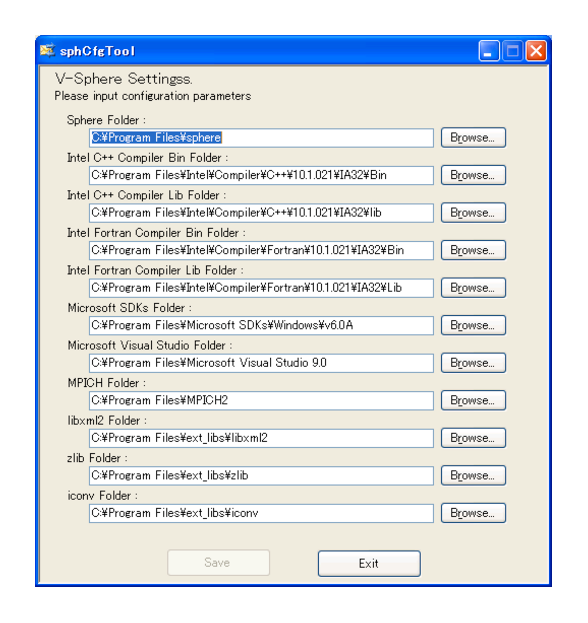
\includegraphics[width=8cm,clip]{sphCfgTool.eps}
\end{center}
\caption{sphCfgToolの設定画面}
\label{fig:sphCfgTool setting}
\end{figure}

\lq\lq sphCfgTool.exe\rq\rq は、インストール中にも起動される.
インストール後は,直接\lq\lq sphCfgTool.exe\rq\rq を起動するか、プログラムメニュー「Sphere」-「sphCfgTool」から起動.
sphCfgToolの画面で,パスの設定が異なっていると赤字\textbf{図\ref{fig:sphCfgTool error}}で\lq\lq Invalid Folder\rq\rq が表示される.
すべてパス設定が行われていることを確認する.

\begin{figure}[htbp]
\begin{center}
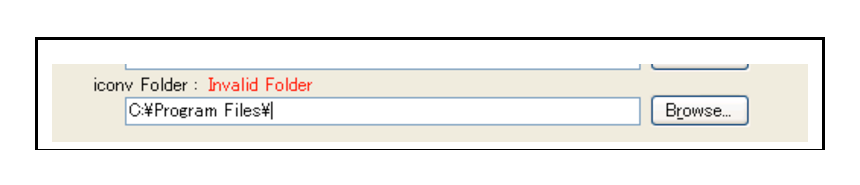
\includegraphics[width=10cm,clip]{error.eps}
\end{center}
\caption{sphCfgToolのパスの設定エラー}
\label{fig:sphCfgTool error}
\end{figure}






%
\chapter{Tips}
\begin{abstract}
コンパイルなどについて役に立つと思われる情報について記す.
\end{abstract}
%

\section{コンパイルエラー}
\label{sec:compile_error}

%
\subsection{VMware上のFedora 14でのコンパイル}
\label{VMware}

\begin{indentation}{3zw}{0zw}
VMware上でFedrora14 32bitがゲストOSの場合,V-Sphere Ver. 1.8.4のコンパイルがうまくいかない場合がある.
その場合,以下の手順で成功する事例がある.

\begin{program}
$ aclocal
$ autoconf
$ automake -a
$ configure [option...]
$ make
\end{program}
\end{indentation}

\subsection{Fedoraにmpich2をインストールした場合のトラブル}
\begin{indentation}{3zw}{0zw}
Linux OSがFedoraで,並列ライブラリとしてmpich2をインストールした場合,
V-Sphereのインストールでリンクエラーとなる場合がある.

その場合,以下のいずれかの手順で成功する事例がある.

\subsubsection{方法1}
mpich2のコンパイララッパーを使用する.

mpich2は、configure時に指定したコンパイラをラップした
コンパイルコマンドがbin配下にインストールされる.

mpich2のインストールディレクトリが/usr/local/mpich2/の場合,/usr/local/mpich2/bin配下に
mpif77,mpif90,mpicc,mpic++等のコマンドが格納されている.
これらのコマンドは、mpich2がintelコンパイラでmakeされて
いれば、内部的にintelコンパイラがコールされ,かつ,MPI
プログラムに必要なライブラリを自動的にリンクしてくれる.

そこで、V-Sphereのconfigure時に,\\
\hspace{1cm}CC=icc\\
\hspace{1cm}CXX=icpc\\
\hspace{1cm}FC=ifort\\
\hspace{1cm}F90=ifort\\
の代わりに,\\
\hspace{1cm}CC=/usr/local/mpich2/bin/mpicc\\
\hspace{1cm}CXX=/usr/local/mpich2/bin/mpic++\\
\hspace{1cm}FC=/usr/local/mpich2/bin/mpif77\\
\hspace{1cm}F90=/usr/local/mpich2/bin/mpif90\\
をそれぞれ指定すると,リンクエラーは解消される.

\subsubsection{方法2}
不足しているライブラリを強制的にリンクする.

mpich2の場合、libmplとlibpthreadをリンクする必要が
あるので,これらのリンク指示をMakefile等に
追記することで,リンクエラーを回避する.

以下のファイルを編集する必要がある.

\paragraph{V-Sphereコンパイル時}
configure実行後に,src/utility/sphDataGather/Makefileの
以下を修正する.\\
218、219行目の「-lmpich」の記述の後に「-lmpl -lpthread」を
追加\\
例)\\
dataGather\_LDADD = -lsphcfg -lmpich -lmpl -lpthread -L/usr/local/mpich2-install/lib -lxml2 -lz -lm\\
sphDataGather\_LDADD = -lsphcfg -lmpich -lmpl -lpthread -L/usr/local/mpich2-install/lib -lxml2 -lz -lm

\paragraph{ソルバープロジェクト(CBC)}
project\_local\_settingsの「LIBS=」の行に「-lmpl -lpthread」を追加\\
(例)\\
LIBS=-lifport -lifcore -lmpl -lpthread

\end{indentation}

\subsection{FedoraにOpenMPIをインストールする場合のトラブル}
\subsubsection{OpenMPIのコンフィギュア}
\begin{indentation}{3zw}{0zw}
Linux OSがFedoraで,並列ライブラリとしてOpenMPIのインストールがうまくいかない場合,OpenMPIのconfigure時に,
\begin{program}
--enable-contrib-no-build=vt
\end{program}
オプションを付加すると,成功する事例がある.
\end{indentation}

\subsubsection{OpenMPIのインストール}
\begin{indentation}{3zw}{0zw}
Linux OSがFedoraで,並列ライブラリとしてOpenMPIをルート権限が必要な場所に
\begin{program}
$ sudo make install
\end{program}
でインストールする場合,
\begin{program}
icc: command not found
\end{program}
というインストールエラーが出る場合がある.\\

その場合,以下の手順で成功する事例がある.\\

rootユーザの.bashrcや.bash\_profielにintelコンパイラのPATHなどの環境設定を記述する.その後,rootユーザとして,
\begin{program}
# make install
\end{program}
\end{indentation}

%
\chapter{アップデート}
\begin{abstract}
本ユーザガイドのアップデート情報について記す.
\end{abstract}
%
%\section{Update}
\label{sec:update info}

%
\subparagraph{Version 1.2.2\hspace{1cm}2011/06/20}
\label{v122}

\begin{description}
\item[-] Windowモジュール作成を追加.
\item[-] 体裁の変更.
\end{description}
\vspace{2mm}

%
\subparagraph{Version 1.2.1\hspace{1cm}2011/06/06}
\label{v121}

\begin{description}
\item[-] OpenMPIをFedoraにインストールするときのオプションをTipsに追記.
\end{description}
\vspace{2mm}

%
\subparagraph{Version 1.2.0\hspace{1cm}2011/05/10}
\label{v120}

\begin{description}
\item[-] Tipsの章を追記.
\end{description}
\vspace{2mm}

%
\subparagraph{Version 1.1.9\hspace{1cm}2011/04/12}
\label{v119}

\begin{description}
\item[-] V-Sphere 1.8.4の機能に対応.
\end{description}
\vspace{2mm}

%
\subparagraph{Version 1.1.8\hspace{1cm}2010/10/31}
\label{v118}

\begin{description}
\item[-] コンパイル環境のアップデートに対応.
\item[-] インストールと開発環境の構築を分離.
\end{description}
\vspace{2mm}

%
\subparagraph{Version 1.1.7\hspace{1cm}2010/10/09}
\label{v117}

\begin{description}
\item[-] 体裁の調整.
\end{description}
\vspace{2mm}

%
\subparagraph{Version 1.1.6\hspace{1cm}2010/07/06}
\label{v116}

\begin{description}
\item[-] MPI2としてOpenMPIのインストールを選択.
\end{description}
\vspace{2mm}

%
\subparagraph{Version 1.1.5\hspace{1cm}2010/05/18}
\label{v115}

\begin{description}
\item[-] LD\_LIBRARY\_PATHのexportの順序を変更.
\end{description}
\vspace{2mm}


%
\subparagraph{Version 1.1.4\hspace{1cm}2010/03/06}
\label{v114}

\begin{description}
\item[-] 「コンフィギュレーション」に用語を統一.
\end{description}
\vspace{2mm}

%
\subparagraph{Version 1.1.3\hspace{1cm}2010/02/10}
\label{v113}

\begin{description}
\item[-] RICCのインストールシェルのコンパイルオプションを-O3
\item[-] V-Sphere 1.7.7の出力に更新.
\item[-] hyperrefを導入.
\end{description}
\vspace{2mm}

%
\subparagraph{Version 1.1.2\hspace{1cm}2010/01/29}
\label{v112}

\begin{description}
\item[-] インストールに失敗した場合の記述を修正.
\item[-] インストールディレクトリの指定について注意書きを追記.
\item[-] 倍精度モジュール時のコメントを追記.
\item[-] インストールに失敗する場合の注意事項を修正.
\item[-] QUESTのIntel Compiler 11.0に変更,Intel mpiを追記.シェルのサンプルを変更.
\item[-] RICCのインストールシェルにLDFLAGSを追記.
\end{description}
\vspace{2mm}

%
\subparagraph{Version 1.1.1\hspace{1cm}2010/01/19}
\label{v111}

\begin{description}
\item[-] OpenMPIを推奨.mpich2の記述を削除.
\item[-] RICCへのインストールを追記.
\end{description}
\vspace{2mm}

%
\subparagraph{Version 1.1.0\hspace{1cm}2010/01/05}
\label{v110}

\begin{description}
\item[-] OpenMPIを推奨.mpich2の記述を削除.
\item[-] mpirunのコメントを追加.
\item[-] 構成変更.sph-cfg.xmlについて追記.
\item[-] ディレクトリ変更に併せて修正.
\end{description}
\vspace{2mm}

%
\subparagraph{Version 1.0.0\hspace{1cm}2009/03/05}
\label{v100}

\begin{description}
\item[-] Version 1.0.0 release
\end{description}
\vspace{2mm}


%
\bibliographystyle{junsrt}
\bibliography{Sphere_UG}

\newpage
\printindex
%
%
\end{document}